

% Prepared by Calvin Kent
%
% Assignment Template v19.02
%
%%% 20xx0x/MATHxxx/Crowdmark/Ax
%
\documentclass[12pt]{article} %
\usepackage{CKpreamble}
\usepackage{CKassignment}
\usepackage{tkz-euclide}
\usepackage{physunits}
\usepackage{physics}
\usepackage{lmodern}
\usepackage{microtype}
\usepackage{upgreek}
\usepackage[misc]{ifsym}


%%Title
\title{\textbf{Assignment 1 Functions - SOLUTIONS} \\ \textbf{Due Date: } Thursday, December 16}
\date{November, 2021}

%%% Maths and science packages

\usepackage{amsmath,amsthm,amssymb}
\usepackage{pgfplots}
	\usetikzlibrary{
		calc,
		patterns,
		positioning
	}
	\pgfplotsset{
		compat=1.16,
		samples=200,
		clip=false,
		my axis style/.style={
			axis x line=middle,
			axis y line=middle,
			legend pos=outer north east,
			axis line style={
				->,
			},
			legend style={
				font=\footnotesize
			},
			label style={
				font=\footnotesize
			},
			tick label style={
				font=\footnotesize
			},
			xlabel style={
				at={
					(ticklabel* cs:1)
				},
				anchor=west,
				font=\footnotesize,
			},
			ylabel style={
				at={
					(ticklabel* cs:1)
				},
				anchor=west,
				font=\footnotesize,
			},
			xlabel= $x$,
			ylabel=$\vec d (\m \tx{[East]})$
		},
	}
	\tikzset{
		>=stealth
	}

%%% Tables and figures packages

\usepackage{float}
\usepackage{caption}
	\captionsetup{
		format=plain,
		labelfont=bf,
		font=small,
		justification=centering
	}


\newcounter{step}[section]
\newenvironment{step}[1][]
{\refstepcounter{step} \textbf{\\Step #1.}}
	
%%% Numbers and sets

\newcommand{\E}{\mathrm{e}}

\newcommand{\tx}[1]{\text{#1}}
\newcommand{\rem}[1]{\operatorname{rem}{(#1)}}


%
\begin{document}
	\pagenumbering{arabic}
	% Start of class settings ...
	\renewcommand*{\coursecode}{MATH 235} % renew course code
	\renewcommand*{\assgnnumber}{Assignment 1} % renew assignment number
	\renewcommand*{\submdate}{September 14, 2021} % renew the date
	\renewcommand*{\studentfname}{Abdullah} % Student first name
	\renewcommand*{\studentlname}{Zubair} % Student last name
    \renewcommand*{\proofname}{Proof:}
	% \renewcommand*{\studentnum}{20836288} % Student number

	\renewcommand\qedsymbol{$\blacksquare$}
	\setfigpath
	% End of class settings	
	% \pagestyle{crowdmark}
	\newgeometry{left=18mm, right=18mm, top=22mm, bottom=22mm} % page is set to default values
	\fancyhfoffset[L,O]{0pt} % header orientation fixed
	% End of class settings
	%%% Note to user:
	% CTRL + F <CHANGE ME:> (without the angular brackets) in CKpreamble to specify graphics paths accordingly.
	% The command \circled[]{} accepts one optional and one mandatory argument.
	% Optional argument is for the size of the circle and mandatory argument is for its contents.
	% \circled{A} produces circled A, with size drawn for letter A. \circled[TT]{A} produces circled A with size drawn for TT.
	% https://github.com/CalvinKent/My-LaTeX
	%%%

	%%%%%%%%%%%%%%%%%%%%%%%%%%%%%%%%%%%%%%%%%%%%%%%%%%%%%%%%%%%%%%%%%%%%%%%%%%%%%%%
	%%%                        CUSTOM MACRO VIM-TEX                             %%%
	%%       call IMAP('NOM', '\nomenclature{}', 'tex')               

	%%%%%%%%%%%%%%%%%%%%%%%%%%%%%%%%%%%%%%%%%%%%%%%%%%%%%%%%%%%%%%%%%%%%%%%%%%%%%%%

	% Crowdmark assignment start
	% qnumber, qname, qpoints
\maketitle
	\section{Preamble}
  This assignment covers everything most of Unit 1. The solutions that you hand in should be \textbf{neat} and \textbf{legible},
  this is an assignment, not a quiz, so I expect you to take your time and present thorough and detailed solutions.
\section{Name and Date:}
	Print your name and todays date below;\\


	\begin{center}
	\noindent\begin{tabular}{ll}
		\makebox[3in]{\hrulefill} & \makebox[3in]{\hrulefill}\\
		Name & Date\\[8ex]% adds space between the two sets of signatures
	\end{tabular}
	\end{center}
	\newpage



\begin{qstn}
  We define the \textbf{cardinality} of sets to be the size of the set, in other words the cardinality of a set is the number of
  elements in the set. For example if $S = \{3,2,1,\triangle \} $, then we say the that cardinality of $S$ is $4$, because  $S$ 
  consists of four elements. The notation we use to describe the cardinality of a set is a pair of bars $(\left|\right|)$ similar to absolute
  values. So going back to our example with  $S$, instead of saying the sentence; The cardinality of  $S$ is $4$, we could
  instead simply write $\left|S\right| = 4$. In this question we will discover that for sets $A,B,C$, it is \textbf{not} always
  true that $\left|A + B\right| = \left|A\right| + \left|B\right|$.

  Lets say we have the following sets,
  \begin{itemize}
    \item $\mathcal{H} = \{x\in \Z \mid -1 \leq x \leq 5\} $
    \item $\mathcal{T} = \{y\in \Z \mid  2 \leq y < 7\} $
  \end{itemize}
  

  \begin{enumerate}[label=(\alph*)]
    \item Write down the elements of both sets.
      \begin{solution}
        \begin{align*}
          \mathcal{H} &= \{-1,0,1,2,3,4,5\}\\
          \mathcal{T} &= \{2,3,4,5,6\} 
        .\end{align*}
      \end{solution}
    \item Determine $|\mathcal{H}|$ and $|\mathcal{T}|$.
      \begin{solution}
        \begin{align*}
          \left|\mathcal{H}\right| &= 7\\
          \left|\mathcal{T}\right| &= 5
        .\end{align*}
      \end{solution}
    \item Determine $|\mathcal{H + T}|$. (Go back to Homework-1 if you forgot how we preform set addition).
      \begin{solution}
        We first determine $\mathcal{H} + \mathcal{T}$,
        \begin{align*}
          \mathcal{H} + \mathcal{T} &= \{-1,0,1,2,3,4,5\} + \{2,3,4,5,6\} \\
                                    &= \{-1,0,1,2,3,4,5,2,3,4,5,6\} \tag{Merge Step}\\
                                    &= \{-1,0,1,2,3,4,5,6\} \tag{Remove duplicates}
        .\end{align*}
        Hence $\left|\mathcal{H} + \mathcal{T}\right| = 8$.
      \end{solution}
    \item Explain why $|\mathcal{H + T}| \neq |\mathcal{H}| + |\mathcal{T}|$.
      \begin{solution}
        Since $ \left|\mathcal{H} + \mathcal{T}\right| = 8$, and $\left|\mathcal{H}\right| + \left|\mathcal{T}\right| = 7 + 5 =
        12$, then clearly $|\mathcal{H + T}| \neq |\mathcal{H}| + |\mathcal{T}|$.
      \end{solution}
  \end{enumerate}
\end{qstn}

\newpage

\begin{qstn}
  Let 
  \begin{align*}
    f(x) &= -2x^2 - 4x + 5\\
    g(x) &= \frac{3}{4}x - 4
  \end{align*}
  \begin{enumerate}[label=(\alph*)]
    \item Compute $f(-2)$ \textbf{and} $g(3)$.
      \begin{solution}
        \begin{align*}
          f(-2) &= -2(-2)^2 - 4(-2) +  5\\
                &= -2(4) + 8 + 5\\
                &= -8 + 8 + 5\\
                &= 5\\
                \\
          g(3) &= \frac{3}{4}(3) - 4\\
               &= \frac{9}{4} - 4\\
               &= \frac{9 - 16}{4}\\
               &= -\frac{7}{4}
        .\end{align*}
      \end{solution}
    \item Compute $f(g(f(0)))$.
      \begin{solution}
        \begin{step}[1]
          Compute $f(0)$,
           \[
                f(0) = -2(0)^2 - 4(0) + 5 = 0 - 0 + 5 = 5
          .\] 
        \end{step}
        \begin{step}[2]
          Compute $g(f(0))$,
           \[
                g(f(0)) = g(5) = \frac{3}{4}(5) - 4 = \frac{15}{4} - 4 = -\frac{1}{4}
          .\] 
        \end{step}

        \begin{step}[3]
            \begin{align*}
              f(g(f(0))) &= f\left( -\frac{1}{4} \right) \\
                         &= -2\left( -\frac{1}{4} \right) ^2 - 4\left( -\frac{1}{4} \right) + 5\\
                         &= -\frac{2}{16} + 1 + 5\\
                         &= -\frac{1}{8} + 6\\
                         &= \frac{47}{8}
            \end{align*}
        \end{step}
      \end{solution}
      \newpage
    \item Provide a \textbf{sketch} of $f$ on the \emph{axis sheet}.
    \item Provide a \textbf{graph} of $g$ on the \emph{axis sheet}.
      \begin{solution}Solution:
        \begin{center}
        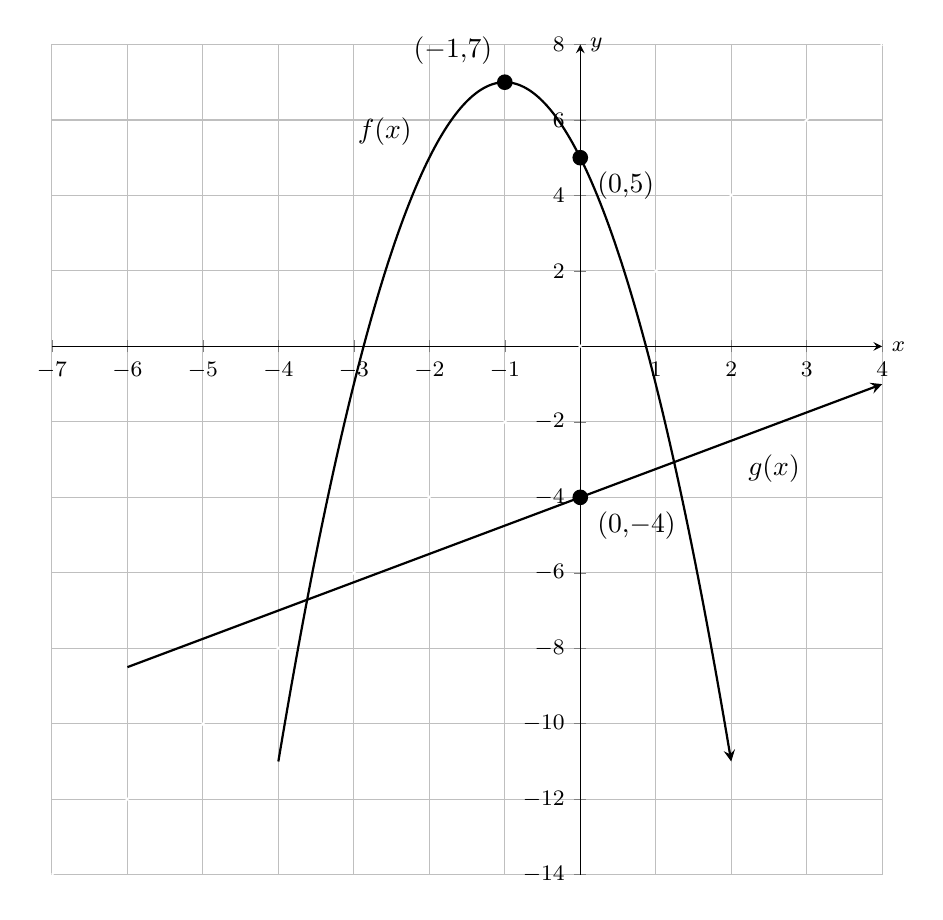
\begin{tikzpicture}
        \begin{axis}[
            my axis style,
            width=\textwidth,
            height=\textwidth,
            ylabel=$y$,
            grid
        ]
        
        \addplot[
            domain=-7:4,
            thick,
            white,
            -
        ]
        {2*x};

        \addplot[
            domain=-4:2,
            thick,
            black,
            ->
        ]
        {-2*x*x - 4*x + 5};

        \addplot[
            domain=-6:4,
            thick,
            black,
            ->
        ]
        {0.75*x - 4};

        \fill[
            black
        ];


        \node[label={110:{($-1$,$7$)}},circle,fill,inner sep=2pt] at (axis cs:-1,7) {};
        \node[label={330:{($0$,$5$)}},circle,fill,inner sep=2pt] at (axis cs:0,5) {};
        \node[label={330:{($0$,$-4$)}},circle,fill,inner sep=2pt] at (axis cs:0,-4) {};
     
        \node[label={160:{$f(x)$}},circle,inner sep=2pt] at (axis cs:-2,5) {};
        \node[label={330:{$g(x)$}},circle,inner sep=2pt] at (axis cs:2,-2.5) {};

        \end{axis}
        \end{tikzpicture}
        \end{center}
      \end{solution}
    \item Does the vertex of $f$ represent a minimum or maximum? Explain your answer.
      \begin{solution}
        The vertex \textbf{does} repersent a maximum since the direction of opening is downwards.
      \end{solution}
  \end{enumerate}

\end{qstn}

\newpage


\begin{qstn} Recall that when you divide two numbers, there will always be a remainder, sometimes the remainder is zero, other
  times it may not be zero, lets take a look at the following examples;
  \begin{itemize}
    \item $\frac{5}{3}$, the remainder is $2$.
    \item $\frac{12}{2}$, the remainder is $0$.
    \item $\frac{4}{7}$, the remainder is $4$. 
  \end{itemize}
  There is a better way to describe the remainder when dividing two numbers, that is to use the following notation,
  \[
        \text{rem}(a,b)
  .\] The output of this is the remainder when dividing $a$ by $b$, so if we repeat our previous examples again using this new
  notation, we would have,
  \begin{itemize}
    \item $\operatorname{rem}(5,3) = 2$
    \item $\operatorname{rem}(12,2) = 0$
    \item $\operatorname{rem}(4,7) = 4$
  \end{itemize}
  The set of all 'positive numbers' is written as,
  \[
        \mathbb N = \{1,2,3,4,5,6,7,\dots\} 
  .\] Now lets define the following function,
  \begin{align*}
    f &\colon \mathbb N \to \mathbb N\\
    f(n) &= \rem{n,2} + 1
  \end{align*}
  Lets take a look at some examples to see how the function behaves,
  \begin{itemize}
    \item $f(4) = \rem{4,2} + 1 = 0 + 1 = 0$
    \item $f(11) = \rem{11,2} + 1 = 1 + 1 = 2$
  \end{itemize}
  Determine the following,
  \begin{enumerate}[label=(\alph*)]
    \item $f(6)$
      \begin{solution}
        \[
            f(6) = \operatorname{rem}(6,2) + 1 = 0 + 1 = 1 
        .\] 
      \end{solution}
    \item $f(15)$
      \begin{solution}
        \[
            f(15) = \operatorname{rem}(15,2) + 1 = 1 + 1 = 2 
        .\] 
      \end{solution}
      \newpage
    \item $f(f(1))$
      \begin{solution}
        \begin{step}[1]
          Compute $f(1)$,
           \[
               f(1) = \operatorname{rem}(1,2) + 1 = 1 + 1 = 2 
          .\] 
        \end{step}
        \begin{step}[2]
          Compute $f(f(1))$,
           \[
               f(f(1)) = f(2) = \operatorname{rem}(2,2) + 1 = 0 + 1 = 1 
          .\] 
        \end{step}
      \end{solution}
    \item The range of $f$.\\
      (Think carefully about this one, have you seen a pattern with the outputs so far?)
      \begin{solution}
        I claim that $\mathcal{R} = \{1,2\} $ is the range.
          \begin{proof}
            If the input number $n$ is even, then since the remainder of an even number divided by two is zero,
            we conclude that,
            \[
                  f(n) = \operatorname{rem}(n,2) + 1 = 0 + 1 = 1 
            .\] 
            Else if the input number $n$ is odd, then since the remainder of an odd number divided by two is one,
            we conclude that,
            \[
                  f(n) = \operatorname{rem}(n,2) + 1 = 1 + 1 = 2 
            .\] This covers every input case and hence we conlcude that all possible outputs (the range) is $\mathcal{R} = \{1,2\}
            $.

           \end{proof}
      \end{solution}
  \end{enumerate}

\end{qstn}


\begin{qstn}
  Determine the Domain and Range of the following functions,
  \begin{enumerate}[label=(\alph*)]
    \item $L(x) = -4x^2 + 8x + 4$
      \begin{solution}
      \begin{align*}
        \mathcal{D} &= \R\\
        \mathcal{R} &= \{y \in \R \mid y \leq 8\} 
      .\end{align*}
      \end{solution}

    \item $R(x) = -50\left|x - 3\right| - 7$
      \begin{solution}
      \begin{align*}
        \mathcal{D} &= \R\\
        \mathcal{R} &= \{y \in \R \mid y \leq -7\} 
      .\end{align*}
      \end{solution}

      \newpage

    \item $Q(x) = \frac{-3}{2x - 4} + \frac{4}{5}$
      \begin{solution}
      \begin{align*}
        \mathcal{D} &= \{x \in \R \mid x \neq 2\} \\
        \mathcal{R} &= \left\{y \in \R \mid y \neq \frac{4}{5}\right\} 
      .\end{align*}
      \end{solution}

    \item $g(x) = 11\sqrt{-3x + 12} + 1$ 
      \begin{solution}
      \begin{align*}
        \mathcal{D} &= \{x \in \R \mid x \leq 4\} \\
        \mathcal{R} &= \left\{y \in \R \mid y \geq 1\right\} 
      .\end{align*}
      \end{solution}

    \item $x^2 + (y + 11)^2 = 4$.
      \begin{solution}
      \begin{align*}
        \mathcal{D} &= \{x \in \R \mid -2 \leq x \leq 2\}\\
        \mathcal{R} &= \{y \in \R \mid -13 \leq y \leq -9\} 
      .\end{align*}
        
      \end{solution}
  \end{enumerate}
\end{qstn}




\end{document}



































